\documentclass[a4paper, 10pt]{article}
%preample
\usepackage{hyperref} %email, automatically link
\usepackage{url}
\usepackage{todonotes}
\usepackage{booktabs}  %tabular package
\usepackage{amsmath} 	%align formular
\usepackage[linesnumbered]{algorithm2e} % algorithm environment
\usepackage[utf8]{inputenc}
\usepackage{makeidx}
\usepackage{multirow}
\usepackage{tikz}

\makeindex

\newtheorem{mydefinition}{Definition}
\newtheorem{mylemma}{Lemma}

%opening section
\title{ISGS \LaTeX { }Beginner's Workshop 
	\\ \LaTeX 2006 - Exercise Sheet \# 1 }
\author{Trung C. Nguyen 
	\\ email \href{mailto:nguyencanhtrung@me.com}{nguyencanhtrung@me.com} }

\begin{document}
	\maketitle
	\tableofcontents
	
	\newpage
	
%-----------------------------------------------------------
% First SECTION
%-----------------------------------------------------------
	\section{Booktabs with Multicolumn \& Multirow}
	\begin{tabular}{cccc}
		\toprule
		1 & 2 & \multicolumn{2}{c}{3} \\
		\multirow{2}{*}{4}& 5 & 6 & 7 \\
		%& 8 \multicolumn{2}{c}{\multirow{2}{*}{9}} \\
		10 & 11 & & \\
		
	\end{tabular}

%-----------------------------------------------------------
% Second SECTION
%-----------------------------------------------------------
	\section{Math}
	\subsection{Alignment}
	
	\begin{align}
		a_1x + a_2x^2 &= 0 \\
		b_1x +b_2x^2 + b_3x^3 &= 0
	\end{align}

	\subsection{Dot-less vector}
		$$\vec{k} = \vec{i} \times \vec{j} $$
		
		or
		\begin{align}
		\vec{k} = \imath \times \jmath \notag
		\end{align}
	\subsection{Golden Ration}
	Two quantities $a$ and $b$ are said to be in the \emph{golden ration $\varphi$}  if
	
	\begin{equation}
			\frac{a}{b} = \frac{a + b}{a} = \varphi
	\end{equation}
	
	By the way: $\varphi = 1 + \frac{1}{\varphi}$
	
	
%-----------------------------------------------------------
% Third SECTION
%-----------------------------------------------------------	
	\section{1+1=2}
	\begin{align}
		1+2 &= 2 \\
		1 &= \ln e \\
		1 &= \sin^2\alpha + \cos^2\alpha \\
		2 &= \sum_{n =0}^{\infty} \frac{1}{2^n} \\
		\ln e +\left(\sin^2 \alpha + \cos^2 \alpha \right) &= \sum_{n=0}^{\infty} \frac{1}{2^n} \\
		1 &= \cosh \varphi \cdot \sqrt{1 -\tanh^2 \varphi} %\\
		%e= \lim\limits_{c\rightarrow\infty} \right[1 + \frac{1}{c}\left]
	\end{align}
%-----------------------------------------------------------
% Third SECTION
%-----------------------------------------------------------	
	\section{Theorem \& Definitions}
	
	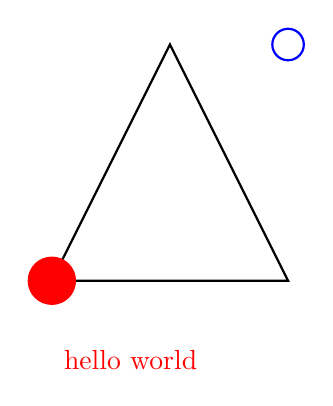
\begin{tikzpicture} 
		\draw[thick] (0,0)--(1.5,3)--(3,0)--cycle; 
		\draw[fill,red] (0,0) circle (3mm);
		\draw[thick,blue] (3,3) circle (2mm); 
		\draw[red] (1,-1) node {hello world}; 
	\end{tikzpicture}
	
	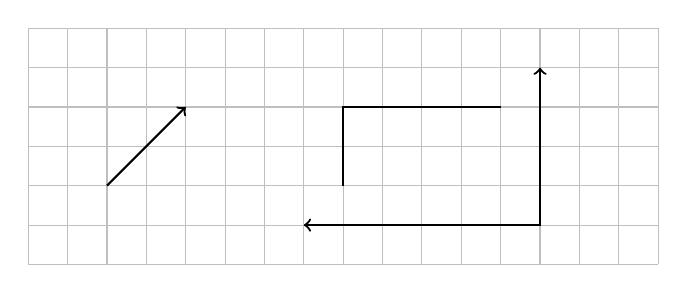
\begin{tikzpicture} 
		\draw[step=0.5,lightgray] (0,0) grid (8,3);  % Grid definition
		\draw[thick,->] (1,1) -- (2,2); 
		\draw[thick,<->] (3.5,0.5) -| (6.5,2.5); 
		\draw[thick] (4,1) |- (6,2); 
	\end{tikzpicture}
	
	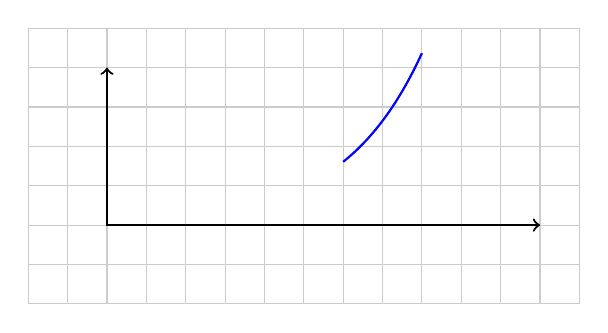
\begin{tikzpicture}%[domain=-0.5:4] 
		\draw[step=0.5,black!20](-1,-1) grid (6,2.5); 
		%\draw[thick,red] plot (\x, {1.5 * sin(\x r)}); 
		\draw[thick,blue, domain = 3:4] plot (\x, {0.04 * exp(\x)}); 
		
		\draw[thick,<->] (0,2)--(0,0)--(5.5,0); 
	\end{tikzpicture}
	
	\begin{mydefinition}
		This is a user defined definition
	\end{mydefinition}	

	\begin{mylemma}
		This is lemma
	\end{mylemma}
\end{document}
